\documentclass[../PianoDiQualifica.tex]{subfiles}
\begin{document}
	\section{Design pattern utilizzati}
		\subsection{Strutturali}
%			\subsubsection{Decorator}
%				\begin{figure}[H] \label{fig:Decorator}
%					\centering
%					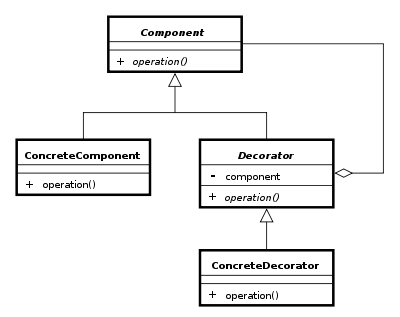
\includegraphics[scale=0.8]{Immagini/DecoratorEx.png}
%					\caption{Esempio pattern Decorator}
%				\end{figure}
%				\paragraph{Scopo\\}
%					Aggiungere responsabilità ad un oggetto dinamicamente.
%				\paragraph{Problema\\}
%					Si vuole aggiungere comportamento o stato ai singoli oggetti durante l'esecuzione
%					e l'ereditarietà non è fattibile perché è statico e si applica ad un'intera classe.
%				\paragraph{Struttura\\}
%					Sono individuabili le seguenti componenti principali:
%					\begin{itemize}
%						\item Component: interfaccia degli oggetti che dovranno essere estesi;
%						\item ConcreteComponent: l'oggetto da estendere;
%						\item Decorator: ha un riferimento all'oggetto Component e
%						definisce un'interfaccia conforme a quella Component;
%						\item ConcreteDecorator: aggiunge funzionalità al Component.
%					\end{itemize}
%				\paragraph{Utilizzo nel progetto\\}
%					% DA AGGIUNGERE (TO DO)
			\subsubsection{Facade}
				\begin{figure}[H] \label{fig:Facade}
					\centering
					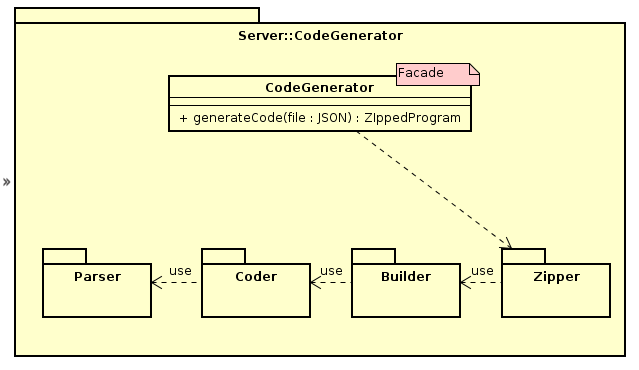
\includegraphics[scale=0.8]{Immagini/FacadeEx.png}
					\caption{Esempio pattern Facade}
				\end{figure}
				\paragraph{Scopo\\}
					Fornire un'interfaccia per l'accesso ad uno o più sottosistemi complessi
					nascondendone la complessità all'esterno.
				\paragraph{Problema\\}
					Una parte del client necessita di una interfaccia semplificata alla funzionalità
					di un sottosistema complesso.
				\paragraph{Struttura\\}
					La principale componente individuabile è la classe Facade che si interpone tra il
					sottosistema e l'esterno, ed associa ogni richiesta ad una classe del sottosistema,
					delegando la risposta.
				\paragraph{Utilizzo nel progetto\\}
					Utilizzato, ad esempio, lato server nel CodeGenerator per interfacciarsi con
					le diverse componenti.
		\subsection{Creazionali}
			\subsubsection{Singleton}
				\begin{figure}[H] \label{fig:Singleton}
					\centering
					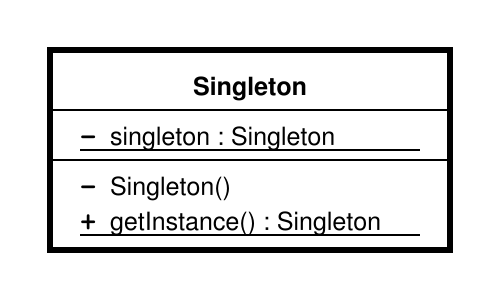
\includegraphics[scale=0.4]{Immagini/SingletonEx.png}
					\caption{Esempio pattern Singleton}
				\end{figure}
				\paragraph{Scopo\\}
					Garantire che venga creata una ed una sola istanza di una determinata classe e di
					fornirne un punto di accesso globale.
				\paragraph{Problema\\}
					Il sistema richiede una ed una istanza di un oggetto; inoltre, sono necessari un
					accesso globale e la possibilità di effettuare un'inizializzazione pigra
					dell'istanza.
				\paragraph{Struttura\\}
					L'unica componente è la classe Singleton che definisce i metodi opportuni per
					permettere la creazione di un'unica istanza e l'accesso a quest'ultima.
				\paragraph{Utilizzo nel progetto\\}
					Utilizzato, ad esempio, lato client per fornire un'unica esistenza della
					classe State interna al Model.
			\subsubsection{Builder}
				\begin{figure}[H] \label{fig:Builder}
					\centering
					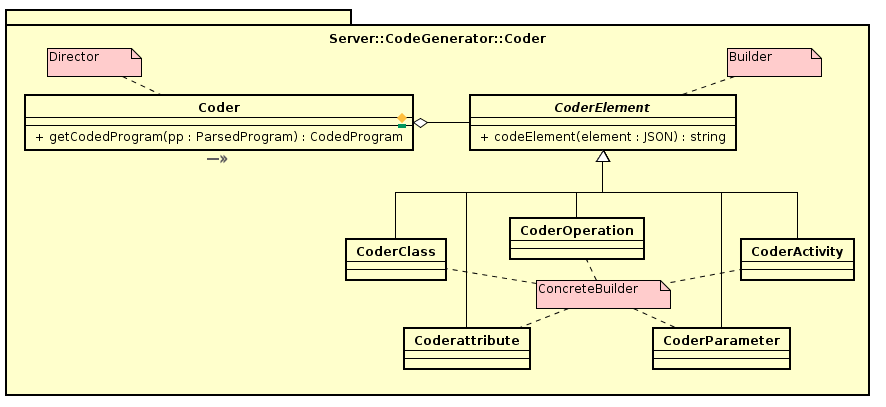
\includegraphics[scale=0.8]{Immagini/Builder.png}
					\caption{Esempio pattern Builder}
				\end{figure}
				\paragraph{Scopo\\}
					Separa la costruzione di un oggetto complesso dalla
					sua rappresentazione.
				\paragraph{Problema\\}
					Necessità di riutilizzare un medesimo algoritmo di
					costruzione per più oggetti di tipo differente.
				\paragraph{Struttura\\}
					Sono individuabili quattro componenti principali:
					\begin{itemize}
						\item Director: Costruisce un oggetto utilizzando il builder (procedura) ;
						\item Builder: Specifica l’interfaccia da utilizzare per assemblare il prodotto;
						\item ConcreteBuilder: Costruisce e assembla le parti del
						prodotto. Tiene traccia dell’istanza costruita. Fornisce un’interfaccia per recuperare il prodotto finale;
						\item Product: Prodotto da costruire.
					\end{itemize}
				\paragraph{Utilizzo nel progetto\\}
					Utilizzato, ad esempio, lato server nella componente Coder per costruire i vari elementi codificati di una classe.
		\subsection{Comportamentali}
			\subsubsection{Observer}
				\begin{figure}[H] \label{fig:Observer}
					\centering
					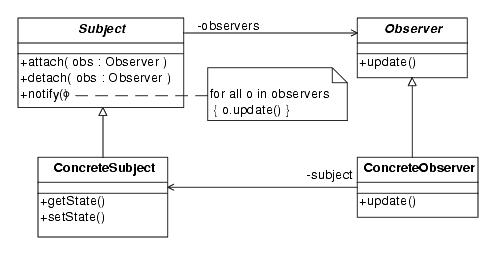
\includegraphics[scale=0.6]{Immagini/ObserverEx.png}
					\caption{Esempio pattern Observer}
				\end{figure}
				\paragraph{Scopo\\}
					Definire una dipendenza "1..n" fra oggetti, riflettendo le modifiche dell'oggetto
					sui suoi dipendenti.
				\paragraph{Problema\\}
					È necessario implementare un sistema di gestione di eventi provenienti da diversi
					oggetti.
				\paragraph{Struttura\\}
					Sono individuabili quattro componenti principali:
					\begin{itemize}
						\item Subject: interfaccia per permettere agli osservatori di sottoscriversi e
						cancellarsi, avendo un riferimento ad ognuno di quelli iscritti;
						\item ConcreteSubject: mantiene lo stato di un oggetto concreto, notificando
						gli osservatori concreti in caso di cambiamenti;
						\item Observer: interfaccia per consentire agli osservatori di aggiornarsi al
						cambiamento di stato dell'oggetto osservato;
						\item ConcreteObserver: implementa l'interfaccia definita dall'Observer
						esplicitando le azioni da eseguire qualora si verifichi un cambio di stato
						dell'oggetto osservato.
					\end{itemize}
				\paragraph{Utilizzo nel progetto\\}
					Utilizzato, ad esempio, lato client dalla View per osservare i cambiamenti del
					Model; la sua implementazione è fornita da Backbone.js.
			\subsubsection{Command}
				\begin{figure}[H] \label{fig:Command}
					\centering
					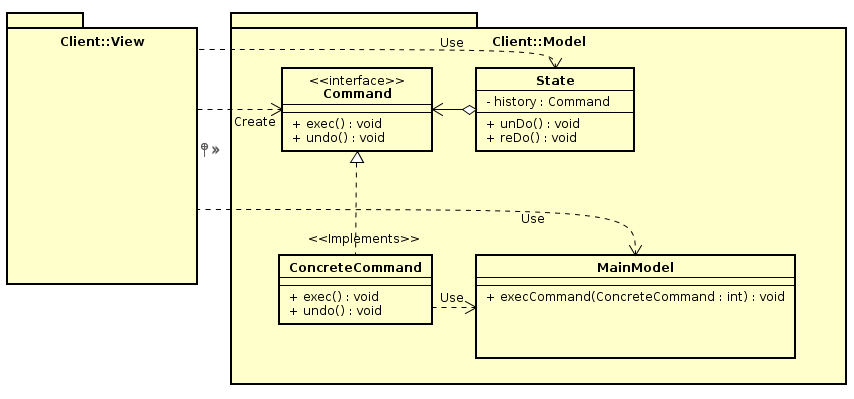
\includegraphics[scale=0.8]{Immagini/CommandEx.png}
					\caption{Esempio pattern Command}
				\end{figure}
				\paragraph{Scopo\\}
					Incapsulare il codice che effettua un'azione separandolo dall'oggetto che ne
					richiede l'esecuzione.
				\paragraph{Problema\\}
					È necessario inviare richieste agli oggetti senza conoscere l'operazione richiesta
					o il destinatario della richiesta.
				\paragraph{Struttura\\}
					Sono individuabili cinque componenti principali:
					\begin{itemize}
						\item Client: effettua la richiesta del comando e imposta il
						Receiver;
						\item Receiver: conosce come effettuare il comando; 
						\item Invoker: effettua l'invocazione del comando;
						\item Command: interfaccia dei comandi;
						\item ConcreteCommand: implementa il comando e invoca l'operazione sul Receiver.
					\end{itemize}
				\paragraph{Utilizzo nel progetto\\}
					Utilizzato, ad esempio, lato client dove ogni intervento della View sul Model sarà
					trasmesso a quest'ultimo attraverso un command avente metodi di "exec()" e "undo()".	
\end{document}